In questo appendice sono riportate alcune immagini prese dall'interfaccia utente del simulatore realizzato. In particolare, in Figura \ref{fig:interface}è riportata l'interfaccia completa del simulatore. Nella parte sinistra è possibile modificare tutti i parametri proposti tramite slider o box di inserimento numerico. Nella parte altra troviamo i pulsanti per avviare, bloccare o ripristinare la simulazione. Sulla destra vi è invece la rappresentazione della mappa e degli agenti robotici.
\begin{figure}
	\centering
	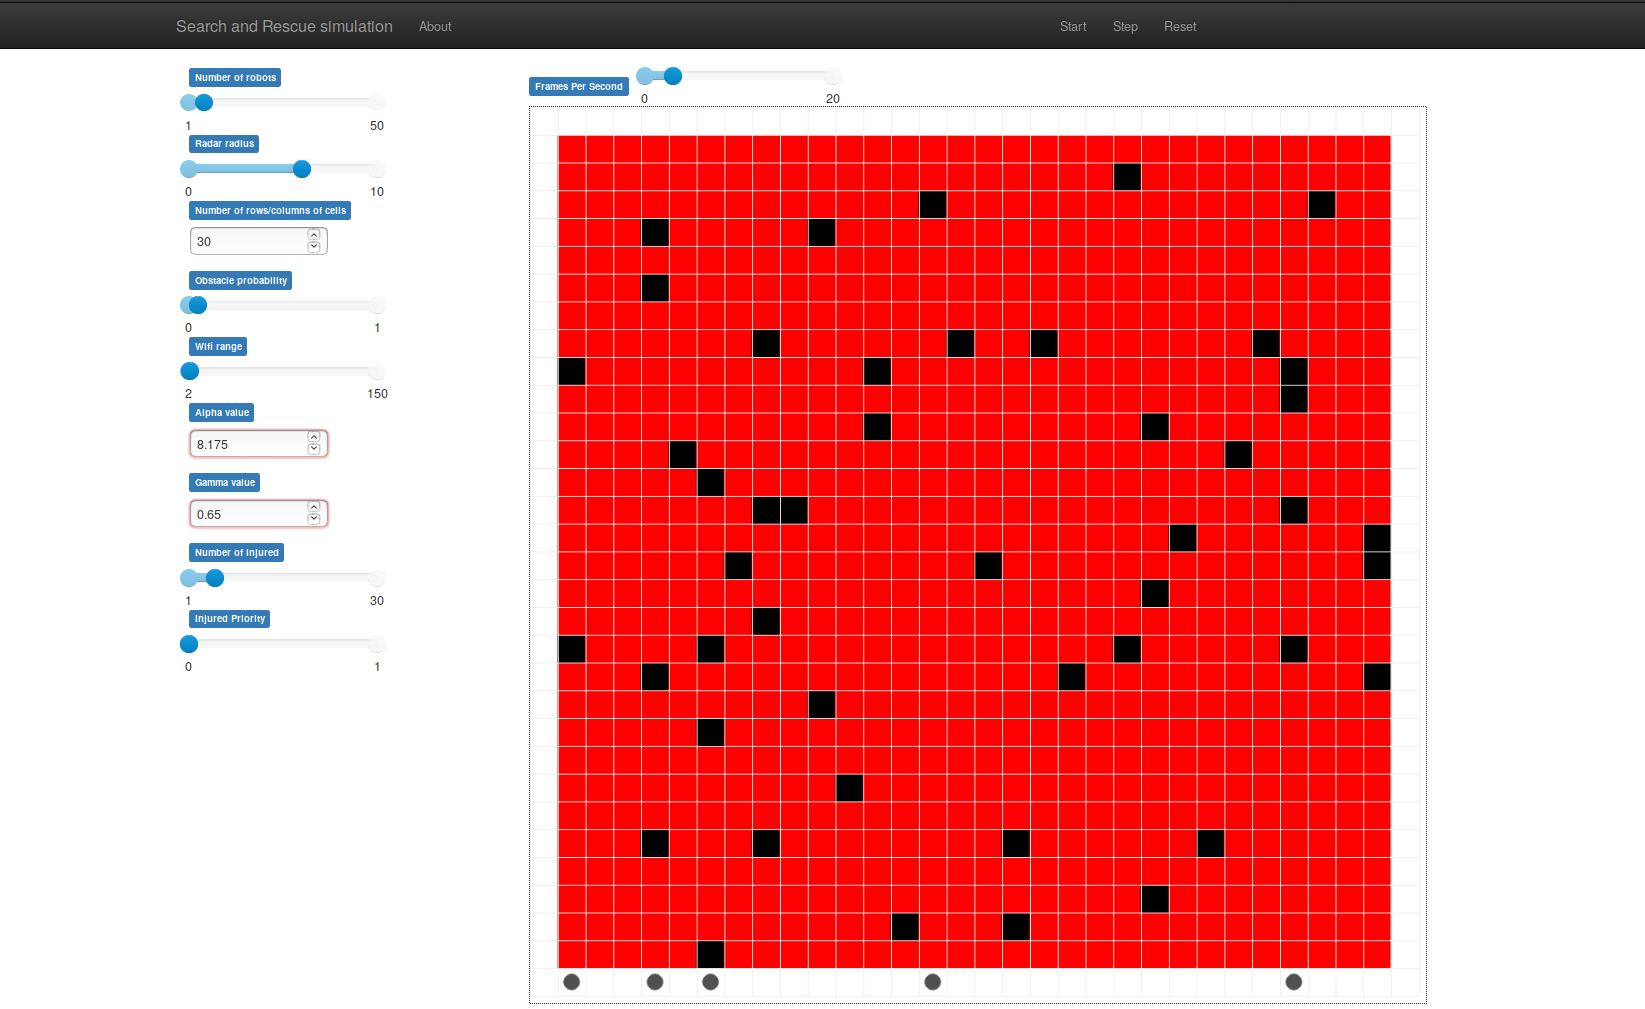
\includegraphics[width=1.2\linewidth]{images/interface}
	\caption{Interfaccia completa del simulatore realizzato.}
	\label{fig:interface}
\end{figure}
In Figura \ref{fig:maps}sono mostrate le 2 mappe denominate \textit{bridge} e \textit{buildings}, rappresentanti rispettivamente una situazione in cui l'area è divisa in due da un fiume non attraversabile e una mappa con grandi edifici crollati e aree irraggiungibili
\begin{figure}
	\subfloat[Mappa rappresentante un'area in cui scorre un fiume con piccoli passaggi.]{
		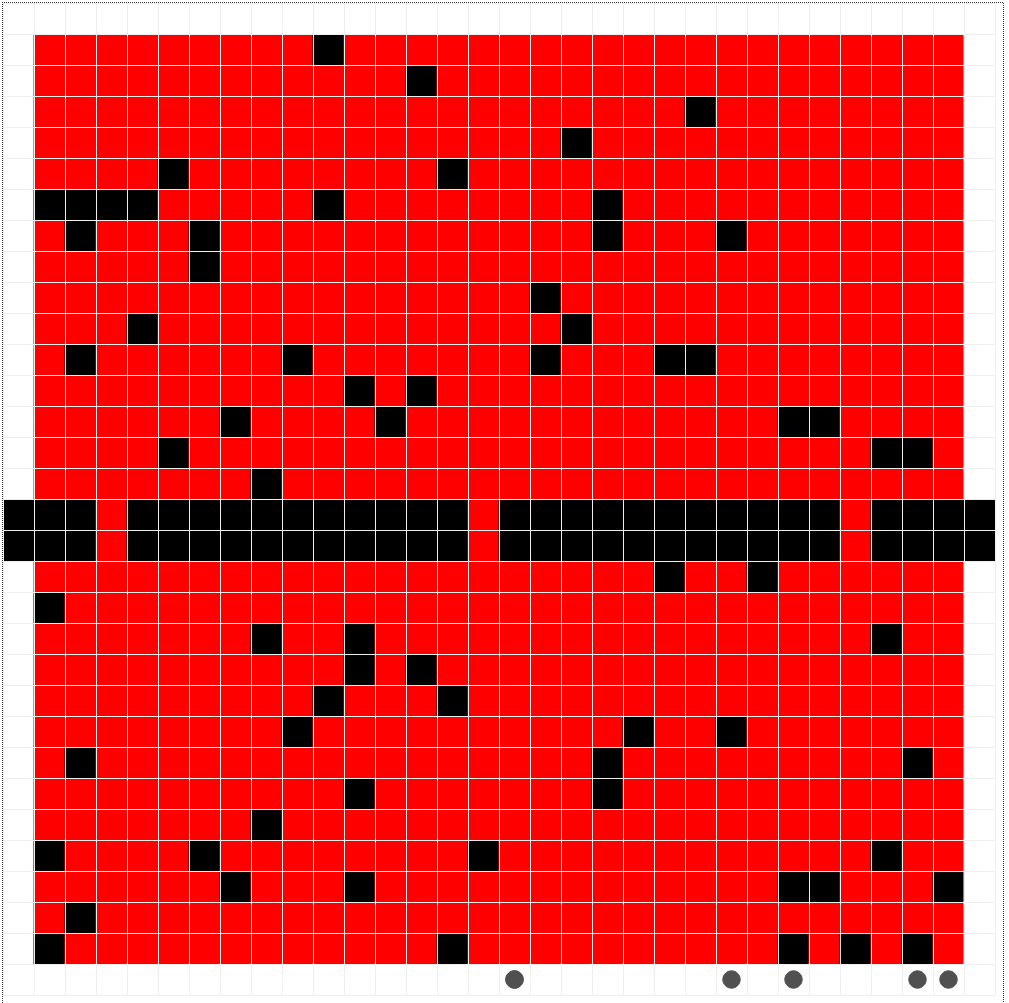
\includegraphics[width=.47\linewidth]{images/bridge}
	}
	\hfill
	\subfloat[Mappa rappresentante un'area in cui sono presenti diversi edifici crollati ed aree irraggiungibili.]{
	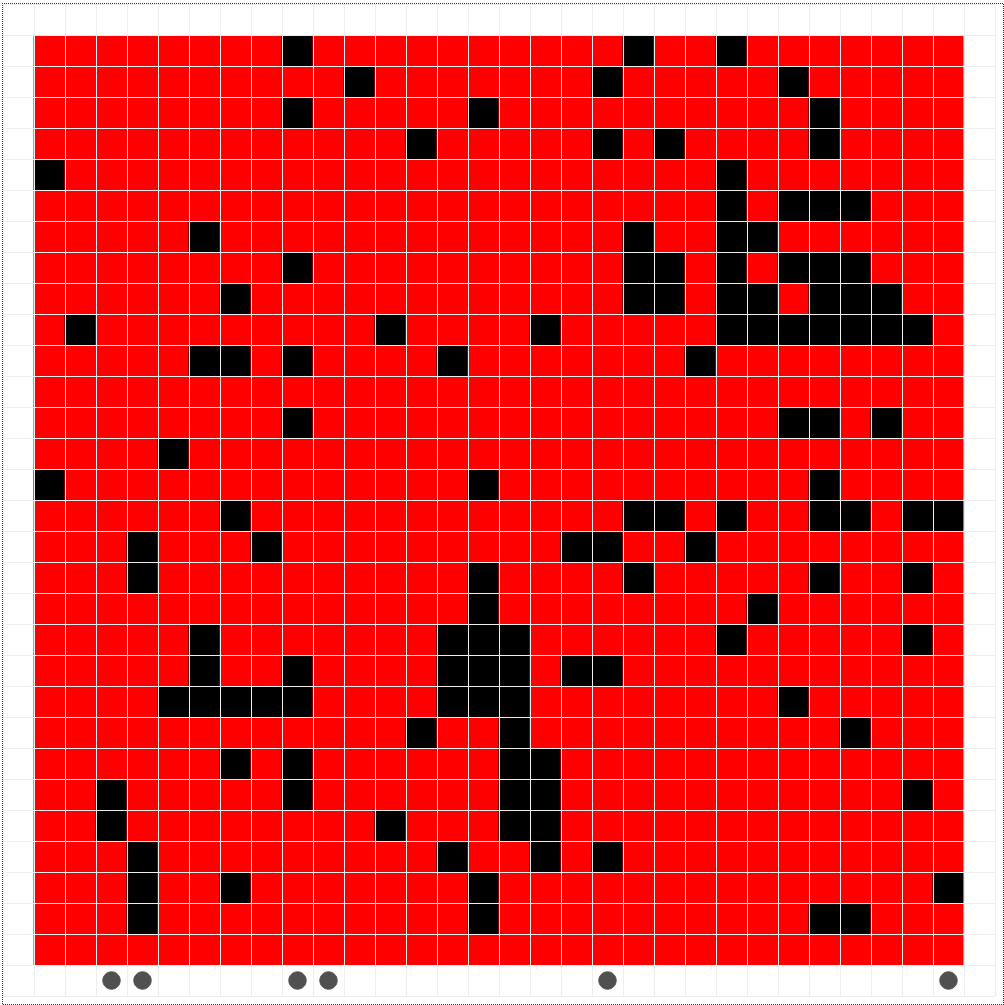
\includegraphics[width=.47\linewidth]{images/buildings}
	}
	\caption{Alcune delle mappe di test utilizzate durante la produzione dei dati.}
	\label{fig:maps}
\end{figure}
Infine, in Figura \ref{fig:explored}, proponiamo la mappa risultante dal processo di esplorazione dei robot con tutti i parametri del simulatore lasciati ai valori di \textit{default}.
\begin{figure}
	\centering
	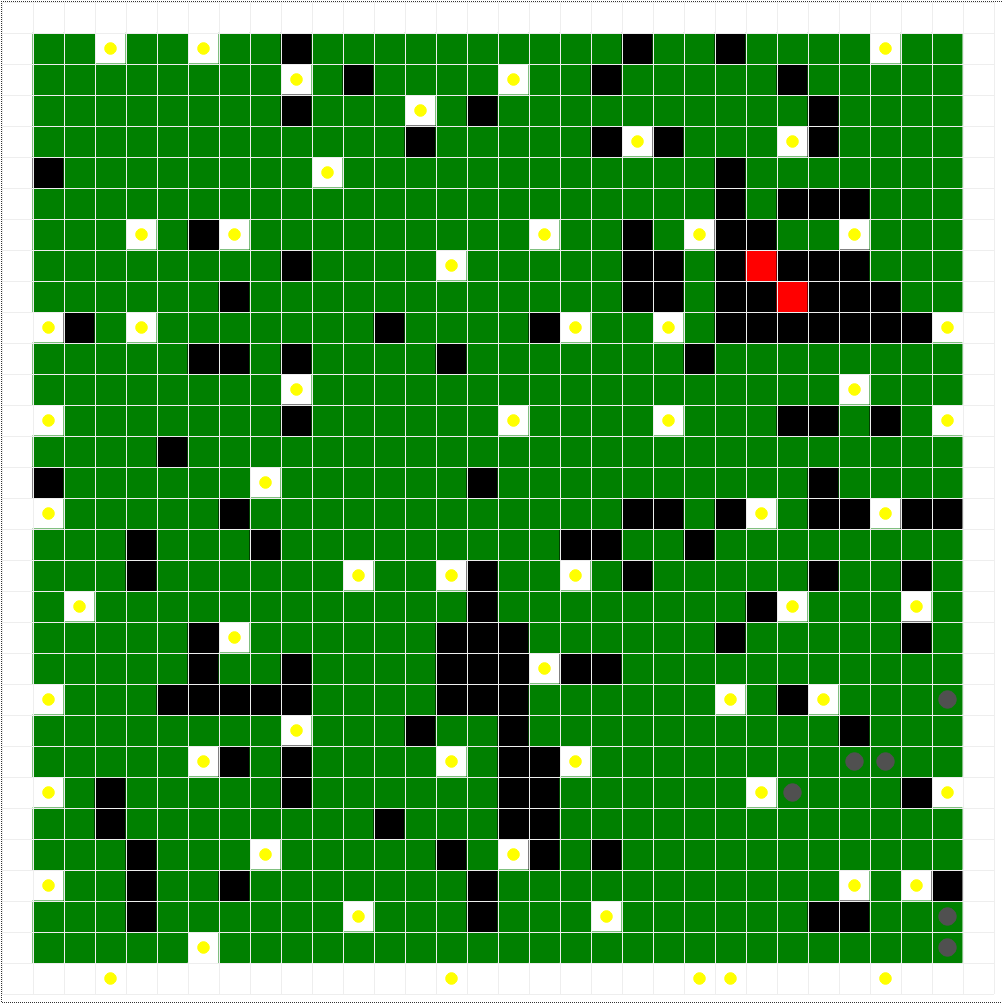
\includegraphics[width=0.8\linewidth]{images/explored}
	\caption{Mappa esplorata al termine della simulazione.}
	\label{fig:explored}
\end{figure}
